
\section{Energy reconstruction}\label{sec:energyreco}
\subsection{Scope of the energy reconstruction}
In this analysis we restrict ourselves to the measurement of the deposited energy in the TPC of the visible particles in the final state of the neutrino interaction. Our signal will have in its final state, by definition, one electron and at least one proton, with no other visible particles. The energy of the electron will be measured by converting the reconstructed charge of all the shower-like objects into deposited energy, as described in Section \ref{sec:showerenergy}. The energy of the protons, instead, can be measured by converting the track length of the reconstructed tracks into deposited energy, using the tabulated stopping power of protons in the liquid argon, with the procedure described in \ref{sec:protonenergy}. The total reconstructed energy will correspond to the sum of the reconstructed energies, corrected by the calibration factors calculated below, and will be referred to as $E_{\mathrm{corr}}$. 


\subsection{Electron energy reconstruction and calibration}\label{sec:showerenergy}
The reconstructed energy $E_{\mathrm{reco}}^{e}$ of a shower-like object is measured converting the charge of the associated hits into deposited energy in the TPC. It is calculated by multiplying the reconstructed charge ($e^{-}_{\mathrm{reco}}$) from hits associated with the reconstructed shower by the calibration factor \cite{michel}:
\begin{equation}
\frac{E_{\mathrm{reco}}^{e} \mathrm{(MeV)}}{e^{-}_{\mathrm{reco}}} = 1.01\frac{e^-}{e^{-}_{\mathrm{reco}}} \times \frac{23.6~\mathrm{eV}}{e^-} \times 10^{-6} \frac{\mathrm{MeV}}{\mathrm{eV}} \times \frac{1}{R} = 3.85\times10^{-5},\label{eq:calib}
\end{equation}
where:
\begin{itemize}

\item the correction factor $1.01\frac{e^-}{e^{-}_{\mathrm{reco}}}$ is obtained measuring the true number of collected electrons $e^{-}$ on the wires using a sample of stopping muons, fitting the $dE/dx$ vs. residual range to values for argon as tabulated by the PDG \cite{pdg};
\item $\frac{23.6~\mathrm{eV}}{e^-}$ is the work function for ionizing an argon atom \cite{workfunction};
\item $R = 0.62$ is the recombination factor obtained with the Modified Box Model \cite{boxmodel} at MicroBooNE's electric field of 270~V/cm.
\end{itemize}

The reconstructed energy is obtained summing the energy of each hit from the reconstructed showers produced by a simulated electron in the collection plane, produced by a $\nu_{e}$ CC0$\pi$-Np interaction. The starting point of the simulated electron and the starting point of the reconstructed showers are required to be within the fiducial volume. 
Figure \ref{fig:ecalib} shows the calibration slope necessary to convert the electron reconstructed energy $E_{\mathrm{reco}}^{e}$ into true electron energy $E^{e}$. The true energy spectrum has been divided in 10 bins of equal size in the 20-2020~Mev range. Since the reconstructed energy distributions in each true energy bin are asymmetric, the data points are obtained fitting the distributions with a GaussExp function \cite{gaussexp}, in order to estimate the most probable value (MPV). The coordinate on the $E^{e}$ axis are given by the mean of the true energy distribution for each bin. The vertical error bars correspond to the full width at half maximum (FWHM) of the fitted function. 

A linear fit of the data points gives:
\begin{equation}
E_{\mathrm{reco}}^{e} = 0.77~E^{e} - 34.7~\mathrm{MeV}.
\end{equation}
The energy of the shower, corrected by the calibration factor is then defined as:
\begin{equation}
E_{\mathrm{corr}}^{e} = (E_{\mathrm{reco}}^{e} + 34.7~\mathrm{MeV})/0.77.
\end{equation}

\begin{figure}[htbp]
\centering
\begin{overpic}[width=0.7\linewidth]{figures/ecalib.pdf}
\end{overpic}
% 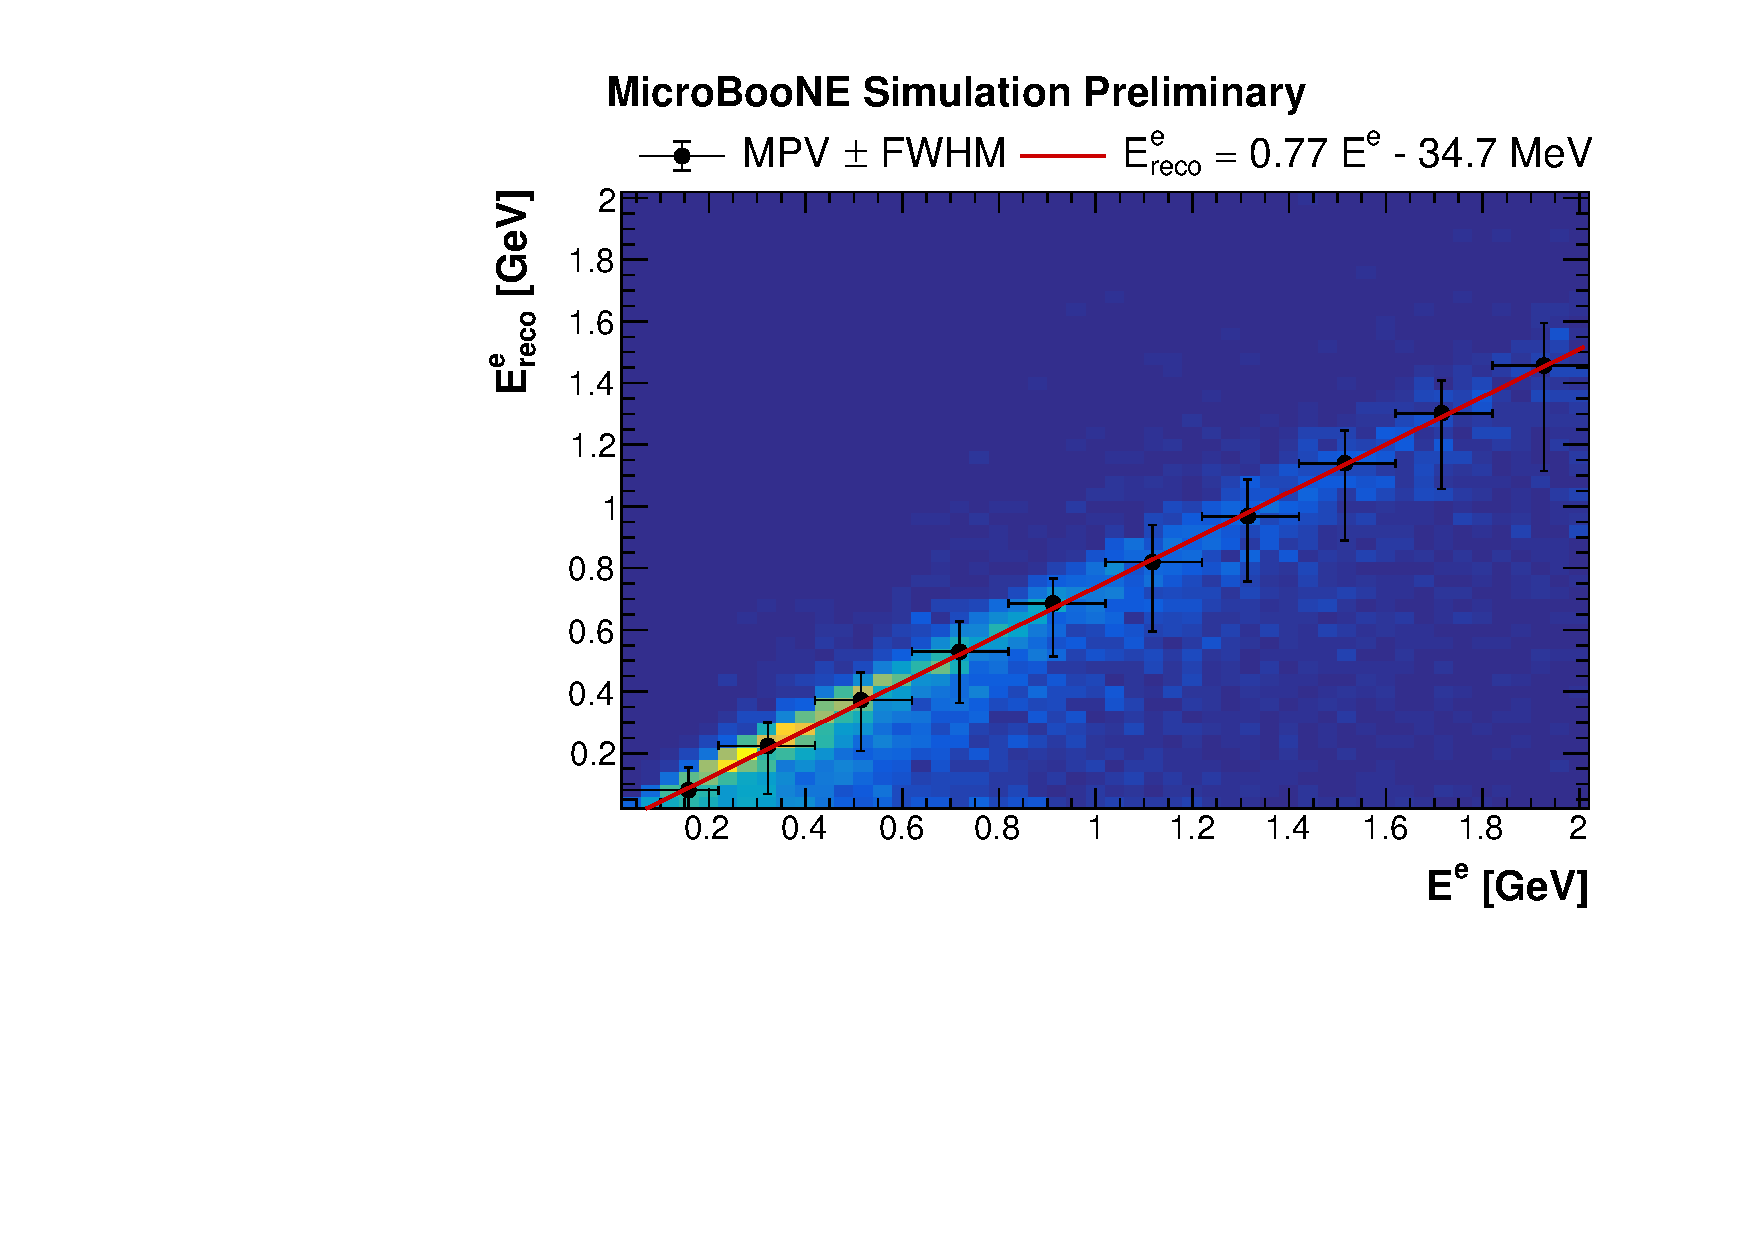
\includegraphics[width=0.65\columnwidth]{figures/ecalib.pdf}
\caption{Bi-dimensional histogram of true electron energy $E^{e}$ vs. reconstructed electron energy $E_{\mathrm{reco}}^{e}$. The reconstructed electron energy is measured summing the energy of each hit associated to reconstructed showers produced by the simulated electron. The black points are obtained measuring the most probable value of the $E_{\mathrm{reco}}^{e}$ distribution for each $E^{e}$ bin, measured by a GaussExp fit}.
\label{fig:ecalib}
\end{figure}

\subsection{Single proton energy reconstruction and calibration}\label{sec:protonenergy}
Proton energy reconstruction is obtained converting the reconstructed track length $L$ into deposited energy using the proton stopping power in liquid argon, as tabulated in \cite{pstar}. Liquid argon density $\rho_{\mathrm{LAr}}$ is assumed to be constant at 1.4~g/ml. Figure \ref{fig:proton} shows the proton kinetic energy as a function of the range of the proton in liquid argon (measured as $L \times \rho_{\mathrm{LAr}}$).

\begin{figure}[htbp]
\centering
  \begin{subfigure}{0.49\textwidth}
  \begin{overpic}[width=\linewidth]{figures/proton.pdf}
\put(120,640){\tiny{\textsf{\textbf{MicroBooNE Simulation Preliminary}}}}
\end{overpic}
%     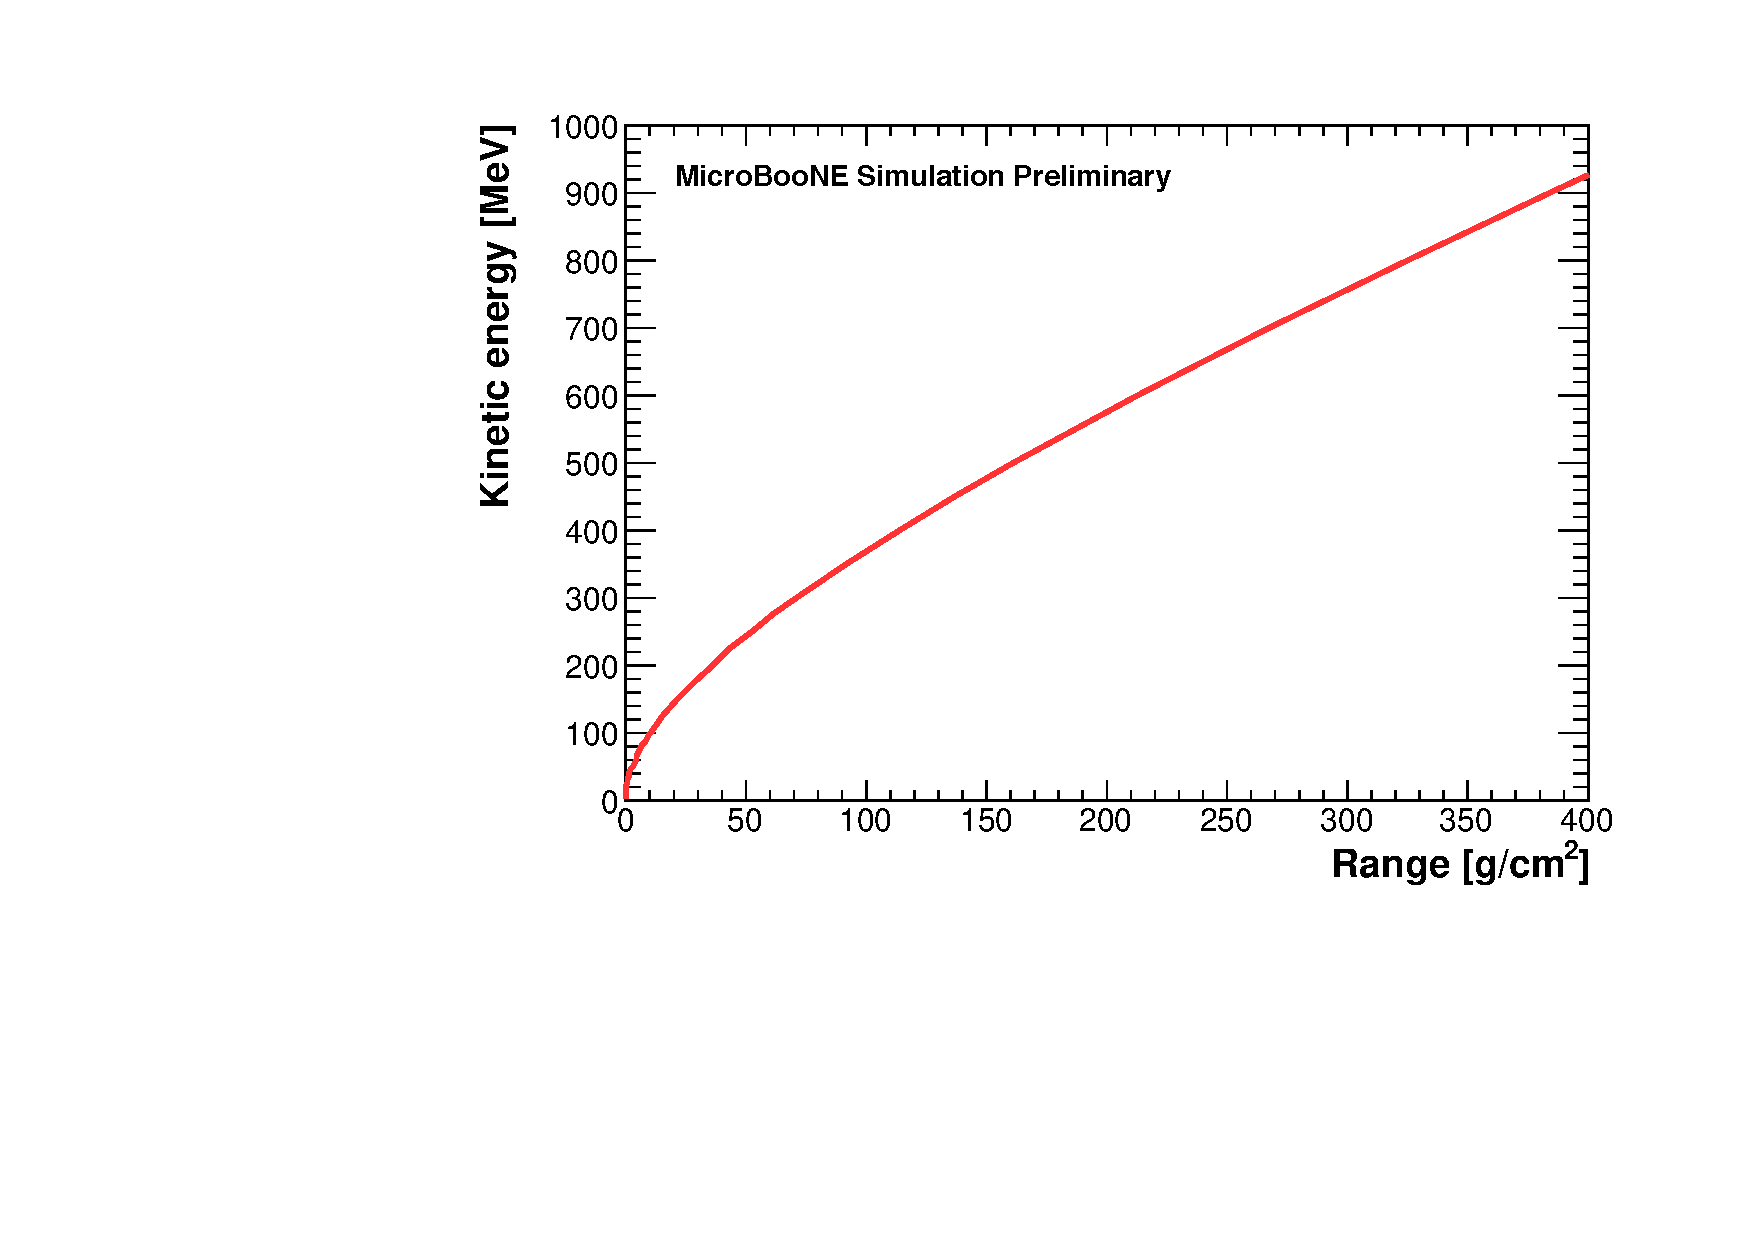
\includegraphics[width=\linewidth]{figures/proton.pdf}
    \caption{Proton kinetic energy as a function of the range of the proton in liquid argon.}\label{fig:proton}
  \end{subfigure}
  \begin{subfigure}{0.49\textwidth}
    \begin{overpic}[width=\linewidth]{figures/pcalib.pdf}\end{overpic}
% 	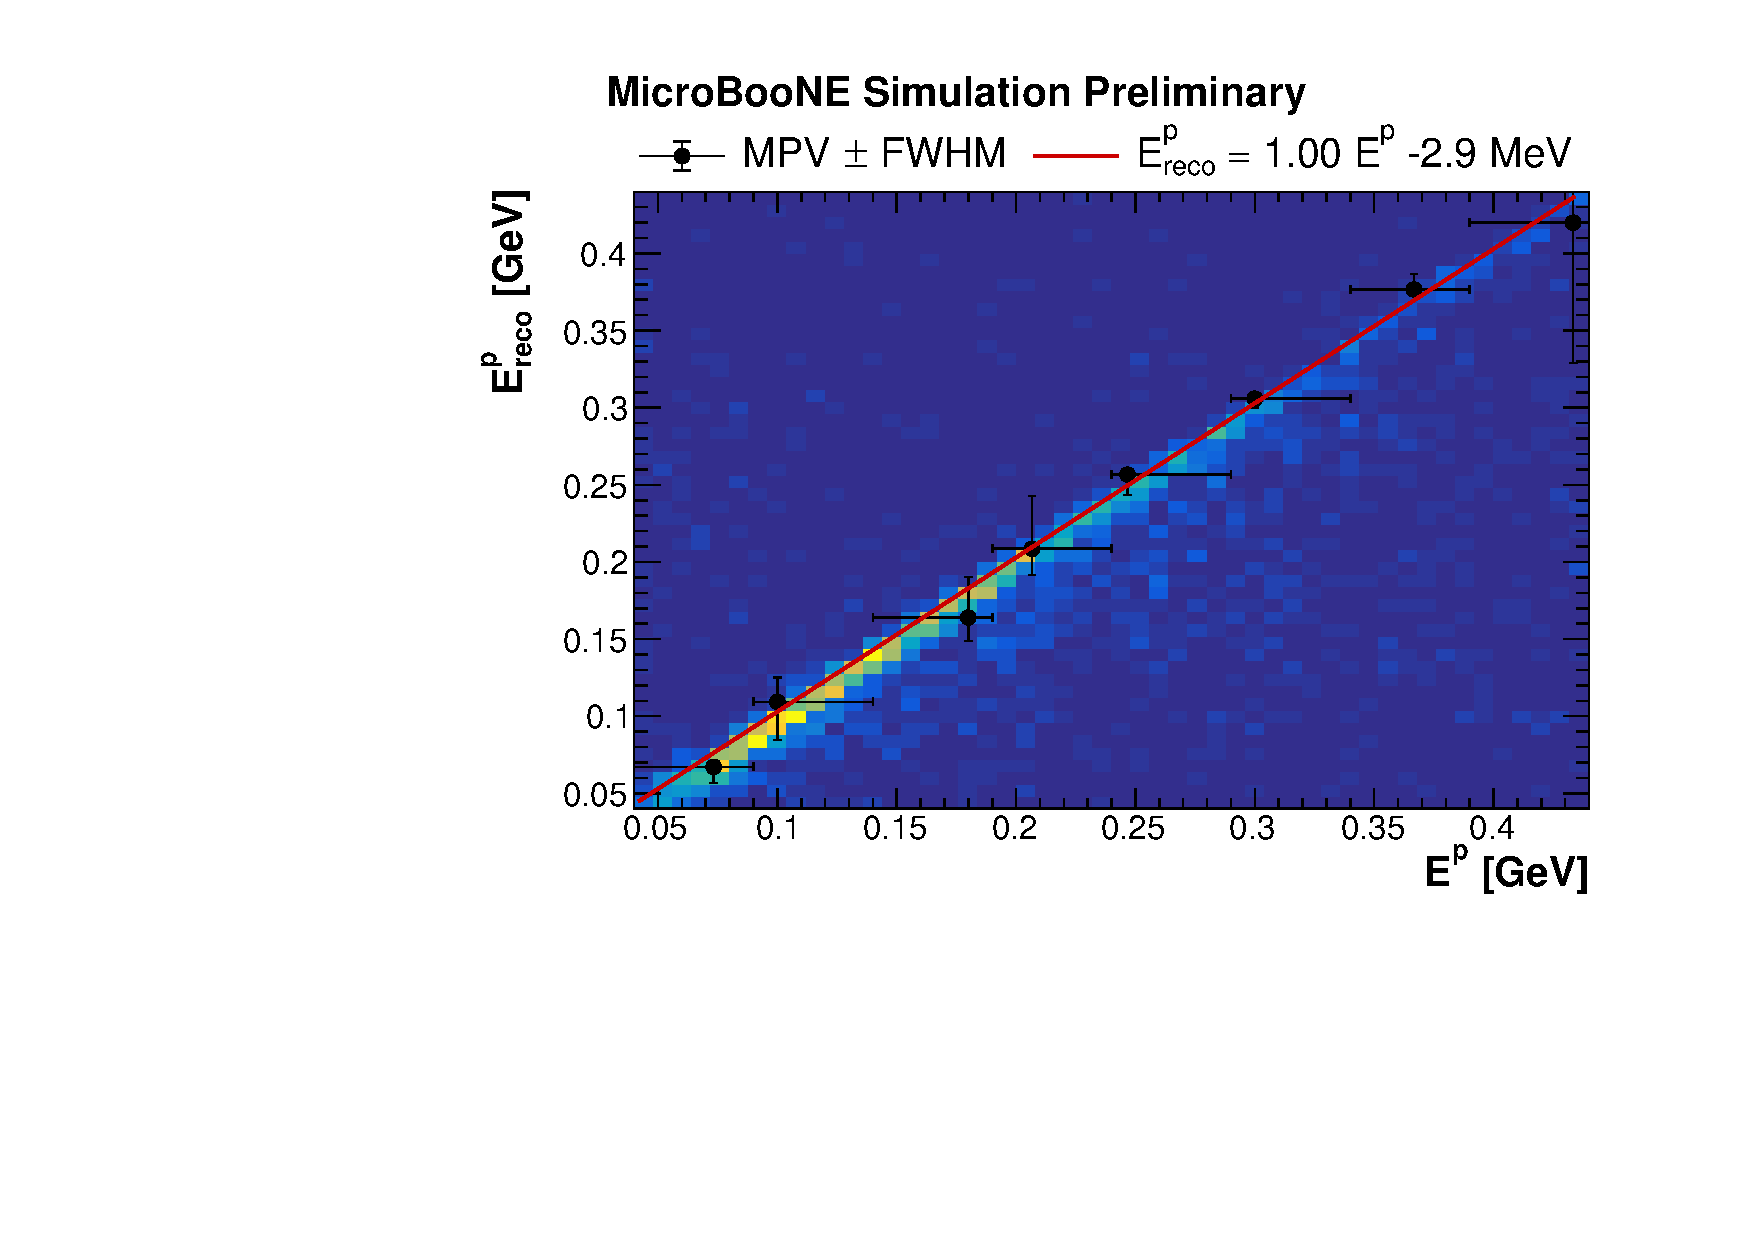
\includegraphics[width=\linewidth]{figures/pcalib.pdf}
     \caption{Bi-dimensional histogram of true proton energy $E^{p}$ vs. reconstructed proton energy $E_{\mathrm{reco}}^{p}$.}\label{fig:pcalib}
   \end{subfigure}
   \caption{The reconstructed proton energy is measured converting the reconstructed track length $L$ into deposited energy using the proton stopping power in liquid argon, as tabulated in \cite{pstar} (left). The calibration is calculated from a linear fit of the most probable values of the $E_{\mathrm{reco}}^{p}$ distribution for each $E^{p}$ bin (right).}
\end{figure}

The calibration constant has been obtained comparing the reconstructed energy of the proton with the true kinetic energy of the simulated proton, in a CC $\nu_{e}$ sample with only one proton in the final state. The true proton and the reconstructed tracks are required to be fully contained within the fiducial volume. Since protons are not minimum-ionizing particles, in the case of two or more tracks (\emph{split tracks}) associated to the same proton, the reconstructed length of the tracks has been summed before calculating the corresponding kinetic energy.
Figure \ref{fig:pcalib} shows the calibration slope necessary to convert the proton reconstructed energy $E_{\mathrm{reco}}^{p}$ into true proton kinetic energy $E^{p}$. For each bin of the true proton energy, the most probable value of the corresponding proton reconstructed energy has been obtained with a GaussExp fit. A linear fit of the data points gives:
\begin{equation}
E_{\mathrm{reco}}^{p} = 1.00~E^{p} - 2.9~MeV.
\end{equation}
The energy of the track, corrected by the calibration factor is then defined as:
\begin{equation}
E_{\mathrm{corr}}^{p} = (E_{\mathrm{reco}}^{p} + 2.9~\mathrm{MeV})/1.00
\end{equation}

\subsection{Deposited Energy Reconstruction}
It is possible to compare the total visible energy in the event $E_{\mathrm{k}}$, defined as the sum of the kinetic energies of the visible particles in the final state, with the sum of the reconstructed energies for shower-like ($E_{\mathrm{corr}}^{e}$) and track-like objects ($E_{\mathrm{corr}}^{p}$) for the selected $\nu_{e}$ CC0$\pi$-Np events. This quantity $E_{\mathrm{corr}}$ is defined as:
\begin{equation}
E_{\mathrm{corr}} = \sum^{N_{p}} E_{\mathrm{corr}}^{p} + \sum^{N_{e}} E_{\mathrm{corr}}^{e},
\end{equation}
where $N_{p}$ is the number of reconstructed tracks and $N_{e}$ is the number of reconstructed showers in the event. For events where we have two or more shower-like objects and no track-like objects, the shower-like object with the lowest proton $\chi^2$ score is chosen as proton candidate. In these cases we have $N_{p} = 1$ by definition.
The reconstructed energy does not include particles that do not interact in the liquid argon (such as neutrons) and charged particles with a kinetic energy below the detection threshold. Figure \ref{fig:nucalib} shows the calibration slope necessary to convert the the total reconstructed energy $E_{\mathrm{corr}}$ into visible energy $E_{\mathrm{k}}$. The plot has been obtained using the $\nu_{e}$ CC0$\pi$-Np + cosmic sample. A linear fit of the data points gives:
\begin{equation}
E_{\mathrm{k}} = 0.98~E_{\mathrm{corr}} - 28.5~\mathrm{MeV}.
\end{equation}
The reconstructed visible energy, corrected by the calibration factor is then defined as:
\begin{equation}
E_{\mathrm{deposited}} = (E_{\mathrm{corr}} + 28.5~\mathrm{MeV})/0.98
\end{equation}

This calibration factor is affected by several factors: among the others, the presence of regions with unresponsive of missing wires can cause an underestimation of the deposited energy. In the future, this effect can be limited by the use of the other two planes for calorimetric measurements.

\begin{figure}[htbp]
\centering
\begin{overpic}[width=0.65\linewidth]{figures/nucalib.pdf}
\end{overpic}\caption{Bi-dimensional histogram of total visible energy $E^{\mathrm{k}}$ vs. the total reconstructed energy $E_{\mathrm{corr}}$. Black points are obtained measuring the most probable value of the $E_{\mathrm{corr}}$ distribution for each $E_{\mathrm{k}}$ bin.} 
\label{fig:nucalib}
\end{figure}

In this analysis, we will use the quantity $E_{\mathrm{deposited}}$ as an estimate of the total visible energy in the event.